\documentclass[11pt,a4paper]{report}
\usepackage[left=3cm,right=3cm, top=3cm]{geometry}

\usepackage{amsmath}
\usepackage{amsfonts}
\usepackage{amssymb}
\usepackage{graphicx}
\usepackage{hyperref}
\usepackage{syntax}
\usepackage{listings}
\usepackage{verbatim}
\usepackage{color}
\usepackage{caption}
\usepackage{url}
\usepackage{cite}
\usepackage[parfill]{parskip}
\usepackage{paralist}
\usepackage{enumitem}
\usepackage{color}
\usepackage[table,xcdraw]{xcolor}
\usepackage{todonotes}
\usepackage{chngcntr}
\usepackage{enumitem}
\usepackage[nottoc,notlot,notlof]{tocbibind}
\usepackage{fancyhdr}

 % Headers and footers
\pagestyle{fancy}
\fancyhf{}
\lhead{}
\chead{}
\rhead{\nouppercase{\leftmark}}
\lfoot{}
\cfoot{\thepage}
\rfoot{}
\renewcommand{\headrulewidth}{0.05pt}
\renewcommand{\chaptermark}[1]{\markboth{\chaptername\ \thechapter.\ \itshape #1}{}}

\setlength{\parindent}{0cm}
\setlength{\parskip}{0.45cm}
\setlist[itemize]{parsep=0.20cm}

\begin{document}

% Bibliography
\bibliographystyle{is-unsrt}
\renewcommand{\bibname}{References}
\counterwithout{figure}{chapter}

\hypersetup{allcolors=black}
\tableofcontents
\newpage

\chapter{Introduction}

Scientists have spent decades building intricate mathematical models for systems and phenomena observed in all areas of life sciences. Such models have greatly expanded our understanding of the complex systems they describe, but the dramatic developments in technology and increase in widely available computational power in recent years have exposed another direction in which current research methodologies can progress.

Simulation in high performance computing environments is today the main approach used to validate scientific models in application domains ranging from astronomy to biomedical or earthquake science. Analytical solutions are often impossible to obtain, given the non-linear nature of these systems, so empirical observations drawn from running them in virtual settings is the only sensible option for further tuning and optimisation.

The prevalence of hypotheses developed by centralising and mining vast arrays of data sources has led to an era of data-centric research \cite{Goble2009}, where powerful cluster, grid and cloud computing platforms are open for scientific usage. However, the expertise required to operate this infrastructure is beyond the skill set of most researchers, so the efficiency of experimentation and the quality of insights drawn from it are heavily influenced by the performance of tools available to manage and process the available data.

\begin{figure}[h]
	\centering
		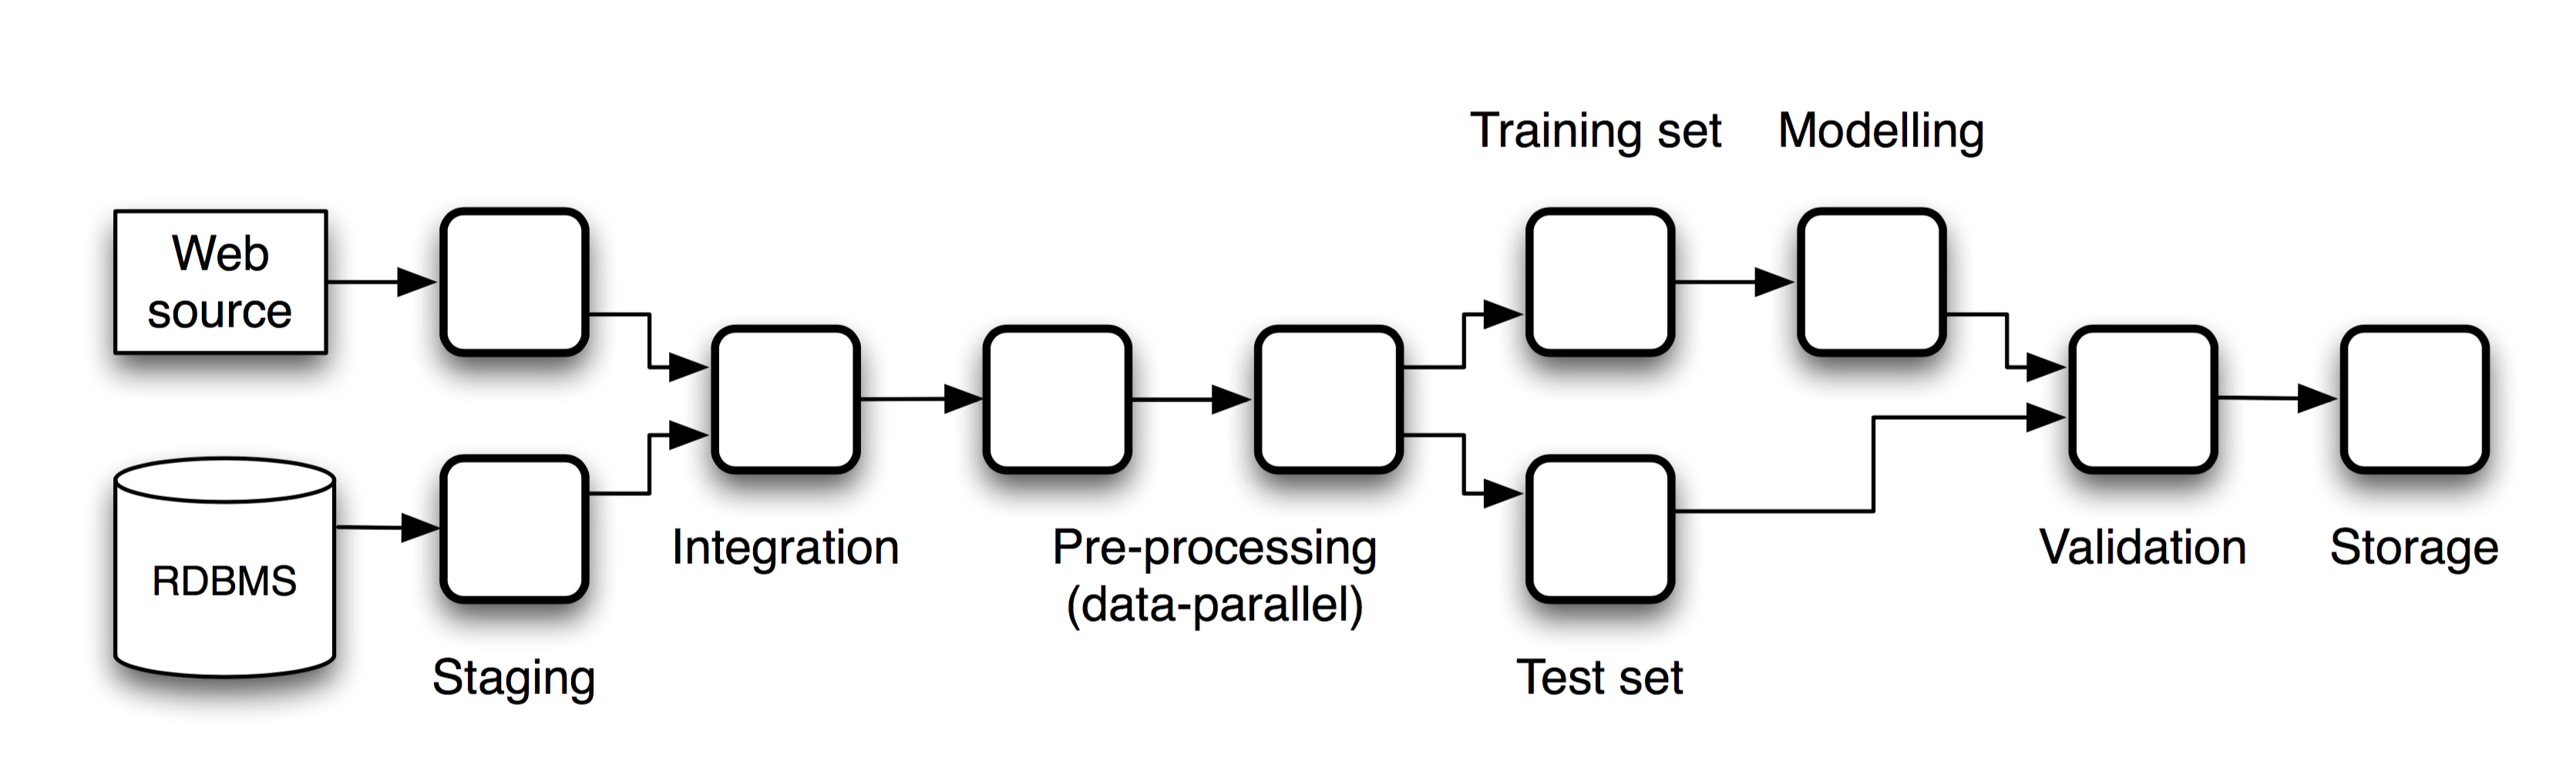
\includegraphics[scale=0.22]{figures/WorkflowExample.png}
	\caption{Workflow example \cite{Curcin2008}.}
	\label{WorkflowExample}
\end{figure}

Workflow management systems provide support for creating data processing pipelines and automating historically tedious tasks such as tuning program parameters by running them repeatedly against many different datasets, defining work units and their interdependencies, or collecting and persisting results of analyses \cite{Goble2009, Taylor2007}. This is all achieved in the context of delegating the work efficiently over resources offered by distributed computing environments.

\section{Motivation}

Although multiple workflow management systems such as Taverna \cite{Taverna}, Kepler \cite{Kepler}, Pegasus \cite{Pegasus} or Galaxy \cite{Galaxy} are already established, many of them focus on specific scientific areas. Since the bioinformatics community is particularly active in adopting the usage of scientific workflows, tools like Galaxy and Kepler have been historically tailored for the needs of researchers in this field.

OpenMOLE \cite{Reuillon2013} is a scientific workflow engine that leverages the natural parallelism of simulation algorithms and targets distributed computing environments to run them. Compared to other existing platforms, OpenMOLE exposes some key features that make it unique:

\begin{itemize}
	\item It is not intended for use within a single scientific community, allowing for generic formalisms that make it general purpose.
	\item It focuses on hiding the complexity and heterogenity of hardware and software infrastructure that grids and cluster provide, separating the workflow definition from the underlying execution environment \cite{Reuillon2010}.
	\item By following a zero-deployment approach, it does not need any guarantees regarding the configuration of its runtime environment. It integrates a standalone packaging system, CARE \cite{Janin2014}, and it ensures reliable execution on remote hosts automatically by copying necessary resources on demand \cite{Reuillon2015}.
	\todo[inline]{@Adrian: I've removed the reference to Yapa (now deprecated) and replaced with CARE, which is the underlying engine of Yapa anyway.}
	\item It treats input models as black-boxes, allowing for interchangeable definitions in diverse languages or even packaged binaries \cite{Reuillon2013}.
	\item The focus on flexible design and scalability generated control flow structures inexistent in most rival platforms. Some of these include loops, conditional branching, or the ability to include whole workflows as subtasks \cite{Reuillon2013}. This makes workflows reusable components that can be published and distributed on the OpenMOLE marketplace \cite{OpenMOLEMarketplace}.
	\item DSL? \todo[inline]{@Adrian: it's definitely an asset for OpenMOLE. Not sure we're the only ones using one though.}
	\item Works with existing applications \todo[inline]{A great advantage of OpenMOLE is you can directly reuse the codes you've developed and are not limited by a pre-configured toolbox}
\end{itemize}


Options that OpenMOLE currently offers to run workflows include:

\begin{itemize}
	\item Multithreading on a local machine.
	\item SSH connections to remote servers.
	\item Grids, such as EGI (European Grid Infrastructure) \cite{EGI}.
	\item Clusters managed by a wide range of software, including PBS (Portable Batch System) \cite{PBS}, Torque \cite{Torque}, SGE (Sun Grid Engine) \cite{SGE}, Slurm \cite{SLURM}, HTCondor \cite{HTCondor}, or OAR \cite{OAR}.
\end{itemize}

However, OpenMOLE does not support distributing the workload on cloud computing environments. at the moment. This is a significant disadvantage compared to other similar applications, since cloud providers are ubiquitous and cheap resources. Providing cloud support will enable a large user base to accelerate their research using OpenMOLE.

\section{Objectives}

The goal of this project is to enhance OpenMOLE by adding the ability to target computing clouds to the arsenal of available execution environments. More specifically, the main objective is to support running jobs on Amazon EC2 \cite{EC2}, as well as on Imperial College's Department of Computing private CloudStack deployment.

\todo[inline]{Change to something like "running jobs on Amazon EC2, while remaining generic enough to potentially target other cloud providers (Google Cloud, OpenStack, ...)}

The key objectives of the project include:

\begin{itemize}
	\item Investigating the APIs and frameworks suitable to instantiate and coordinate computations on cloud infrastructures. In accordance with OpenMOLE's philosophy, we will favour Free and Open Source technologies. Initial steps involve researching the cloud distribution architecture of similar open source scientific workflow engines, as well as industrial software.
	\item Implementing a solution using the chosen tools as part of GridScale \cite{Passerat2016}, the engine powering OpenMOLE's distributed computation service. The library already has a modular structure, so development should be possible in isolation from the rest of the already production-ready modules.
	\item Fully automating the process of provisioning and and bootstrapping individual machines or clusters in the cloud. This should be invisible to the end user so that the only required configuration steps are entering the access credentials for the respective cloud and possibly setting up limits on resource consumption in order to avoid excessive costs.
	\item Evaluating the new environment against Amazon EC2 and the department's cloud, comparing its performance to benchmarks for already supported grids and clusters and, possibly, other workflow management systems. Comparison with other similar systems is considered a stretch goal, since the evaluation process would be tedious by requiring to define the work units for each system independently and results are likely to be spurious, since they might be caused by limitations in other parts of the system. Benchmarking performance between the cloud and a grid given the performance specifications of instances in both environments is expected to give more valuable results under these conditions.
\end{itemize}

\todo[inline]{@Jonathan: We insist on not only allowing to run jobs in cloud environments, but actually allowing to run them on clusters in the cloud. Most other workflow systems do not really make a distinction at this level and they instead say they support EC2 if they have an AMI that allows running the job on an EC2 instance. However, I'm not sure why we necessarily need a cluster, since EC2 already has robust autoscaling features. Is it because we want to parallelise the execution of tasks and this can not be achieved by a machine being autoscaled to a larger capacity? Would it also be the case that an extra machine could not be used as effectively as when for example using instances as servers for client requests, since a long-running job filling up the capacity of an instance can not be simply split up midway through execution?}

\todo[inline]{If the above is the case, useful references to automatic upscaling and downscaling depending on load can be found in "Scientific Workflow Applications on Amazon EC2" and the Pegasus papers - especially the 2016 one}.


\chapter{Background}

This chapter gives an overview of the current state of the workflow engine ecosystem by looking at some of the existing platforms with a focus on the execution environments they support, and cloud deployments in particular. Next, we describe GridScale, the library used by OpenMOLE to access distributed computing resources and present some basic ideas to enhance it with support for a cloud infrastructure. This leads to the last section, where we investigate tools and frameworks that could allow scheduling of jobs on a cluster of instances provisioned from a cloud.

\section{Grids and Cloud Computing}

\todo[inline]{@Jonathan: I was thinking of giving an overview of what the similarities and differences between grids and clouds are, as I was myself confused in the beginning - probably a short description of EC2 and CloudStack  and a writeup of something similar to these articles: http://www.cloud-lounge.org/clouds-and-grids-compared.html and http://www.ibm.com/developerworks/library/wa-cloudgrid/. Is it worth it?}

\todo[inline]{Can use Pegasus papers for a nice comparison from the point of view of workflow management systems.}

\section{Workflow Platform Ecosystem}

Chronologically, scientific workflow systems have emerged from the bioinformatics community along with the recent trend towards data-driven research. Their large number and segregation despite achieving similar purposes could be explained by many research groups independently trying to formalise, consolidate and generalise their workflows. Therefore, most systems achieve comparable goals, with slight variations. Common features include \cite{Goble2009}:

\begin{itemize}
	\item Creation and definition of reusable tasks or work units. A task can represent anything from processing an image to running an expensive computation or invoking a service over the web.
	\item A graphical user interface that simplifies the flow of tasks by allowing definitions via a simple visual representation. See Figure \ref{OpenMOLEGUI} for an example of this.
	\item An execution platform that runs the workflow, hiding the complexity of calling service applications, managing and storing data, setting up and consuming remote computational resources, dealing with failures and logging results and unexpected behaviours. This is the engine of the application.
	\item A collaboration platform, where users can interact and share workflows.
\end{itemize}

\begin{figure}[h]
	\centering
		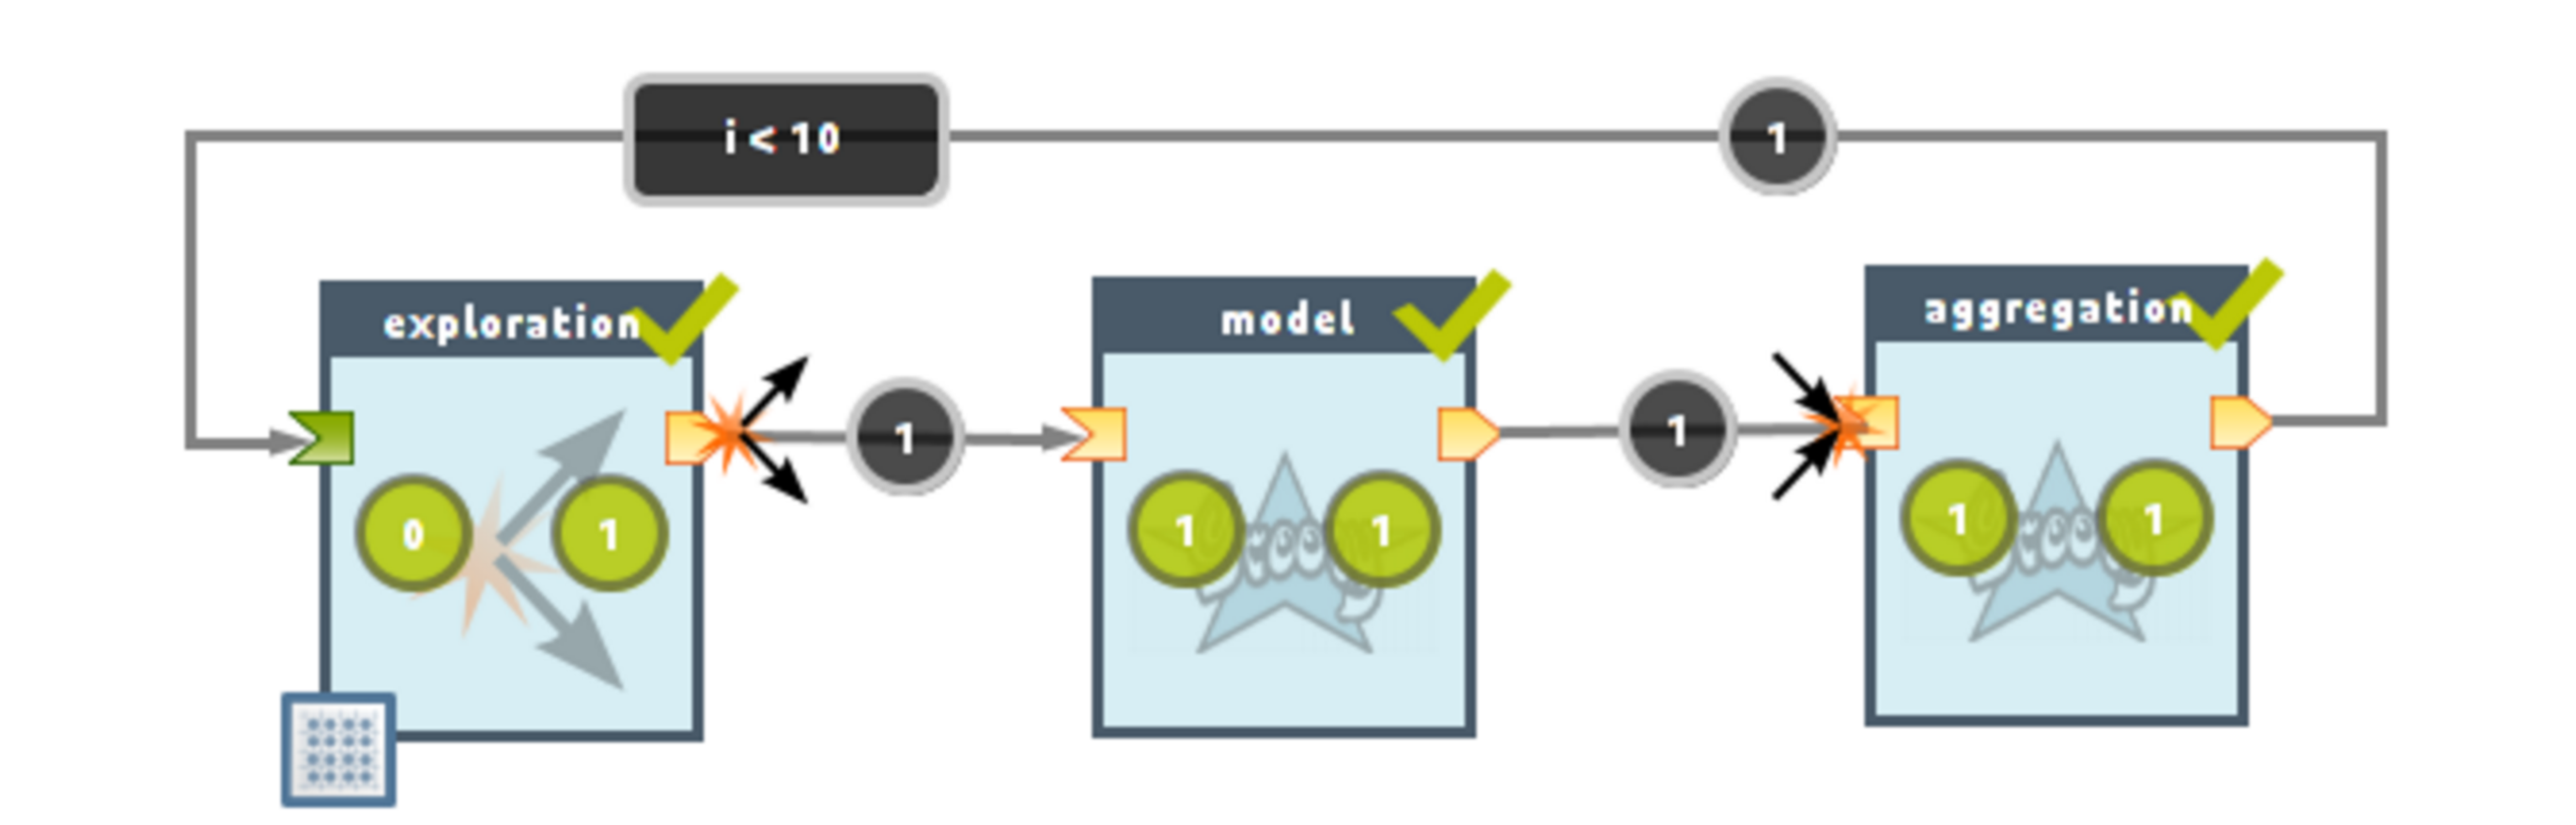
\includegraphics[scale=0.30]{figures/OpenMOLEGUI.png}
	\caption{OpenMOLE graphical workflow \cite{Reuillon2012}.}
	\label{OpenMOLEGUI}
\end{figure}

From the multitude of existing workflow systems, we have selected some of the most often referenced ones for closer inspection. Since our focus only spans the targeting of different remote execution platforms, we will generally omit the details of workflow definition and the underlying implementation, as well as the graphical design and collaboration factors. We are particularly interested in engines that support cloud environments and insights we can draw from their design and infrastructure.

\subsection{Taverna}

Taverna \cite{Wolstencroft2013} is one of the most popular workflow systems. It was initially created as a framework for bioinformatics research and has remained used primarily in this field despite efforts from contributors towards expansion to other research areas.

The system has three main functional components:
\begin{itemize}
	\item \textit{Taverna Workbench} is the standard suite including the user interface and execution platform. However, this package alone is quite restricted since it only supports running the workflow locally and not distributing it remotely.
	\item \textit{Taverna Server} is a suite that works on the principles of simple client-server interaction. A server instance stores workflow blueprints created by the community and the client is only allowed to trigger runs of the experiments via a web interface. In this model, only server administrators have permission to add workflow content, while regular users are not allowed to freely create and upload their own custom workflows to the server. Additionally, the need for a full installation and configuration of the server software in order to execute work remotely limits ease of deployment and creates an important entry barrier.
	\item \textit{Taverna Player} is the web interface used by the client to send requests to Taverna Server.
\end{itemize}

Despite its maturity, Taverna does not, on its own, have built-in support for automatic server installations on grids or clouds. Instead, users need to develop custom orchestration infrastructure for these environments to allow deploying clusters coordinated by the instance where Taverna Server is installed. Both caGrid \cite{caGrid} and BioVeL \cite{BioVeL} have implemented such solutions \cite{TavernaGrid, Donvito} to take advantage of grid resources. On Amazon EC2, Taverna is only available as an Amazon Machine Image (AMI) runnable on a single instance, without support for distributed execution.

\subsection{Galaxy}

Galaxy \cite{Goecks2010} is another community specific web-based platforms for managing workflows, focussing on genomic research. Conceptually, it is driven by the motivation to ensure accessibility of computational resources by providing researchers with simple web interfaces to interact with distributed environments, reproducibility of experiments by tagging and recording order and intent of each action users take, as well as transparency of findings by consolidating a robust collaboration framework.

CloudMan \cite{Afgan2010} is the cloud resource management tool used by Galaxy to instantiate pre-packaged clusters on Amazon EC2 machines. To achieve this, the user needs to use the AWS Management Console to request from an instance that will be used as the master node of a new SGE cluster. Next, the number of slave instances in the cluster can be adjusted using the CloudMan Console, as shown in Figure \ref{CloudManConsole}. Since EC2 instances do not save data on disk by default, persistence on Amazon Elastic Block Storage (EBS) can be explicitly turned on from the CloudMan Console.

\todo[inline]{@Adrian: in the introduction where you plan to compare grids and clouds, it might be worth having a subsection to define Amazon specific terminology: EC2, S3, EBS, ...}

\begin{figure}[h]
	\centering
		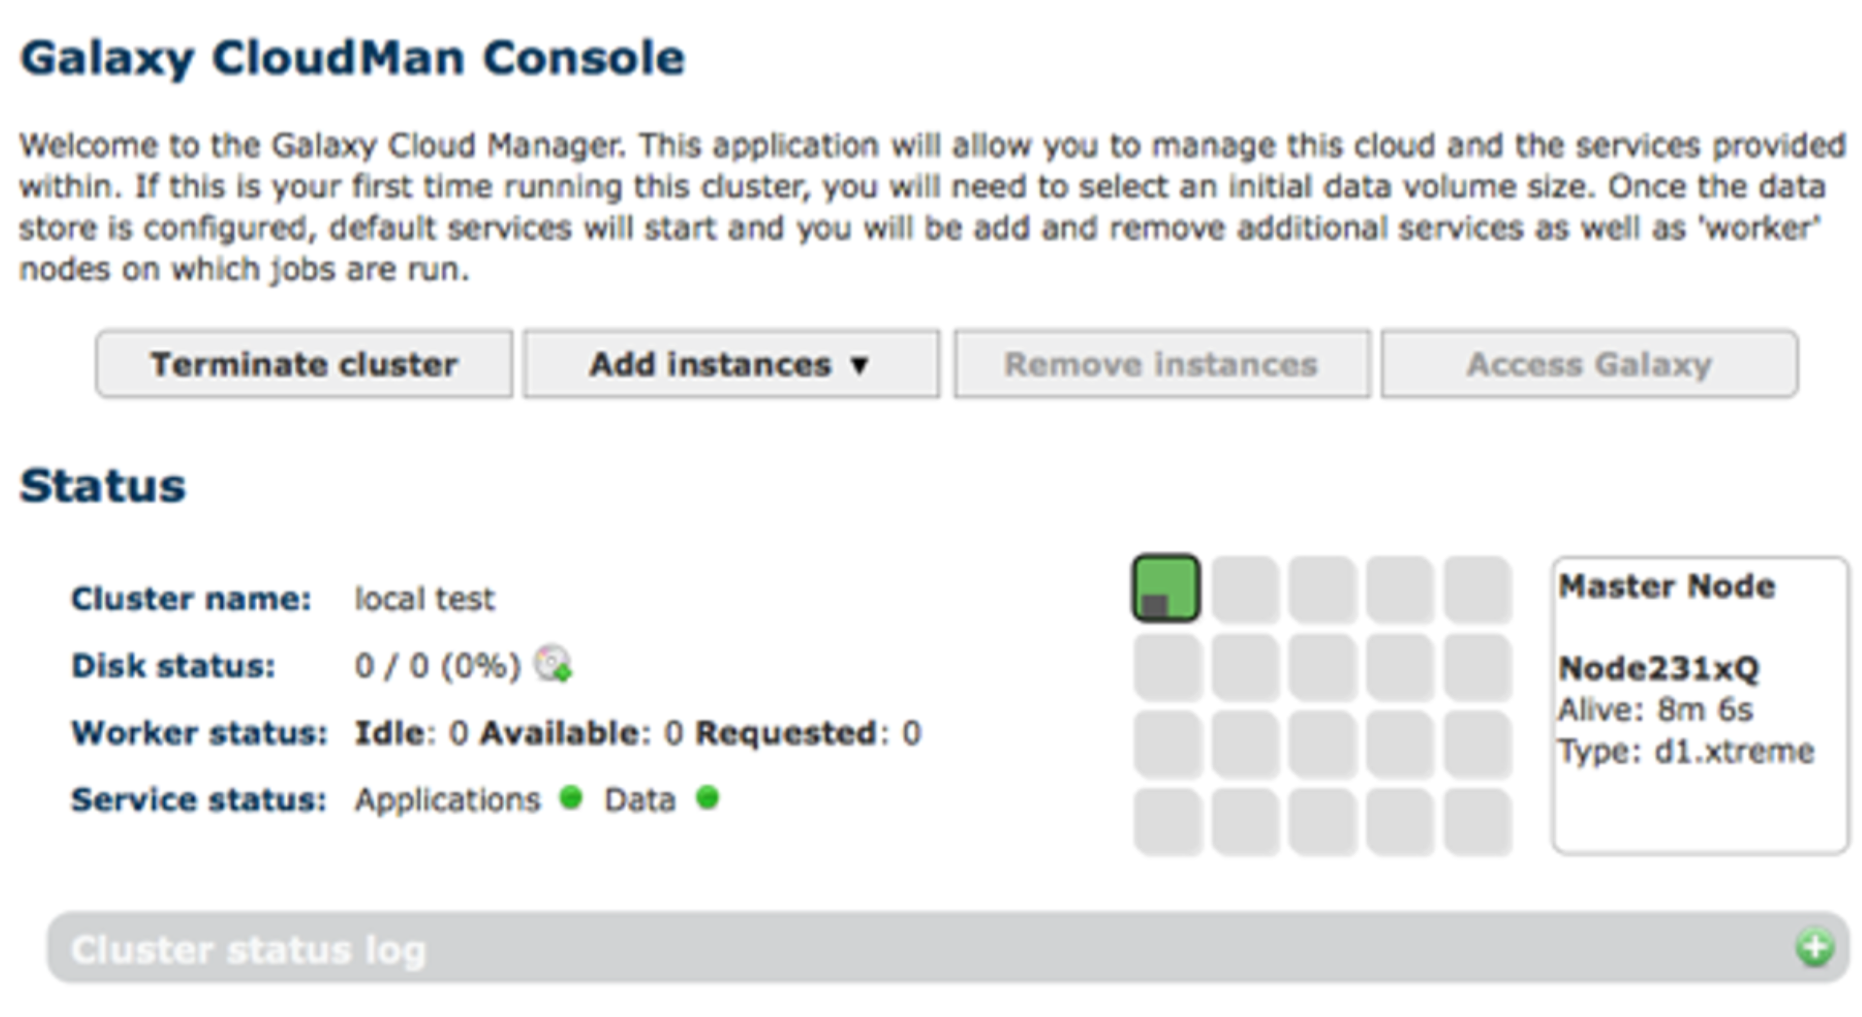
\includegraphics[scale=0.40]{figures/CloudManConsole.png}
	\caption{CloudMan cluster management console \cite{Afgan2010}.}
	\label{CloudManConsole}
\end{figure}

CloudMan also deals with cases when the initial capacity of an EBS volume attached to the master instance is exceeded by safely pausing activity in the cluster before reattaching a new expanded capacity volume and resuming work. However, the job submission system still does not achieve full automation, since it requires a human to manually turn on the master node in the cluster, as opposed to the system being brought up on the fly and turned off on workflow termination.

\todo[inline]{This is a major problem when using commercial clouds, as it means the user keeps on being charged for resources he's not really using anymore}


One major advantage of CloudMan is its modular architecture, under which instances only use a lightweight AMI and reference the tools they need from external storage such as EBS, as shown in Figure \ref{CloudManArch}. This grants further flexibility in terms of updating the system, because the AMI does not need to be repackaged frequently and the state of machines can be modified by simply writing on persistent storage.

\vspace{5mm}
\begin{figure}[h]
	\centering
		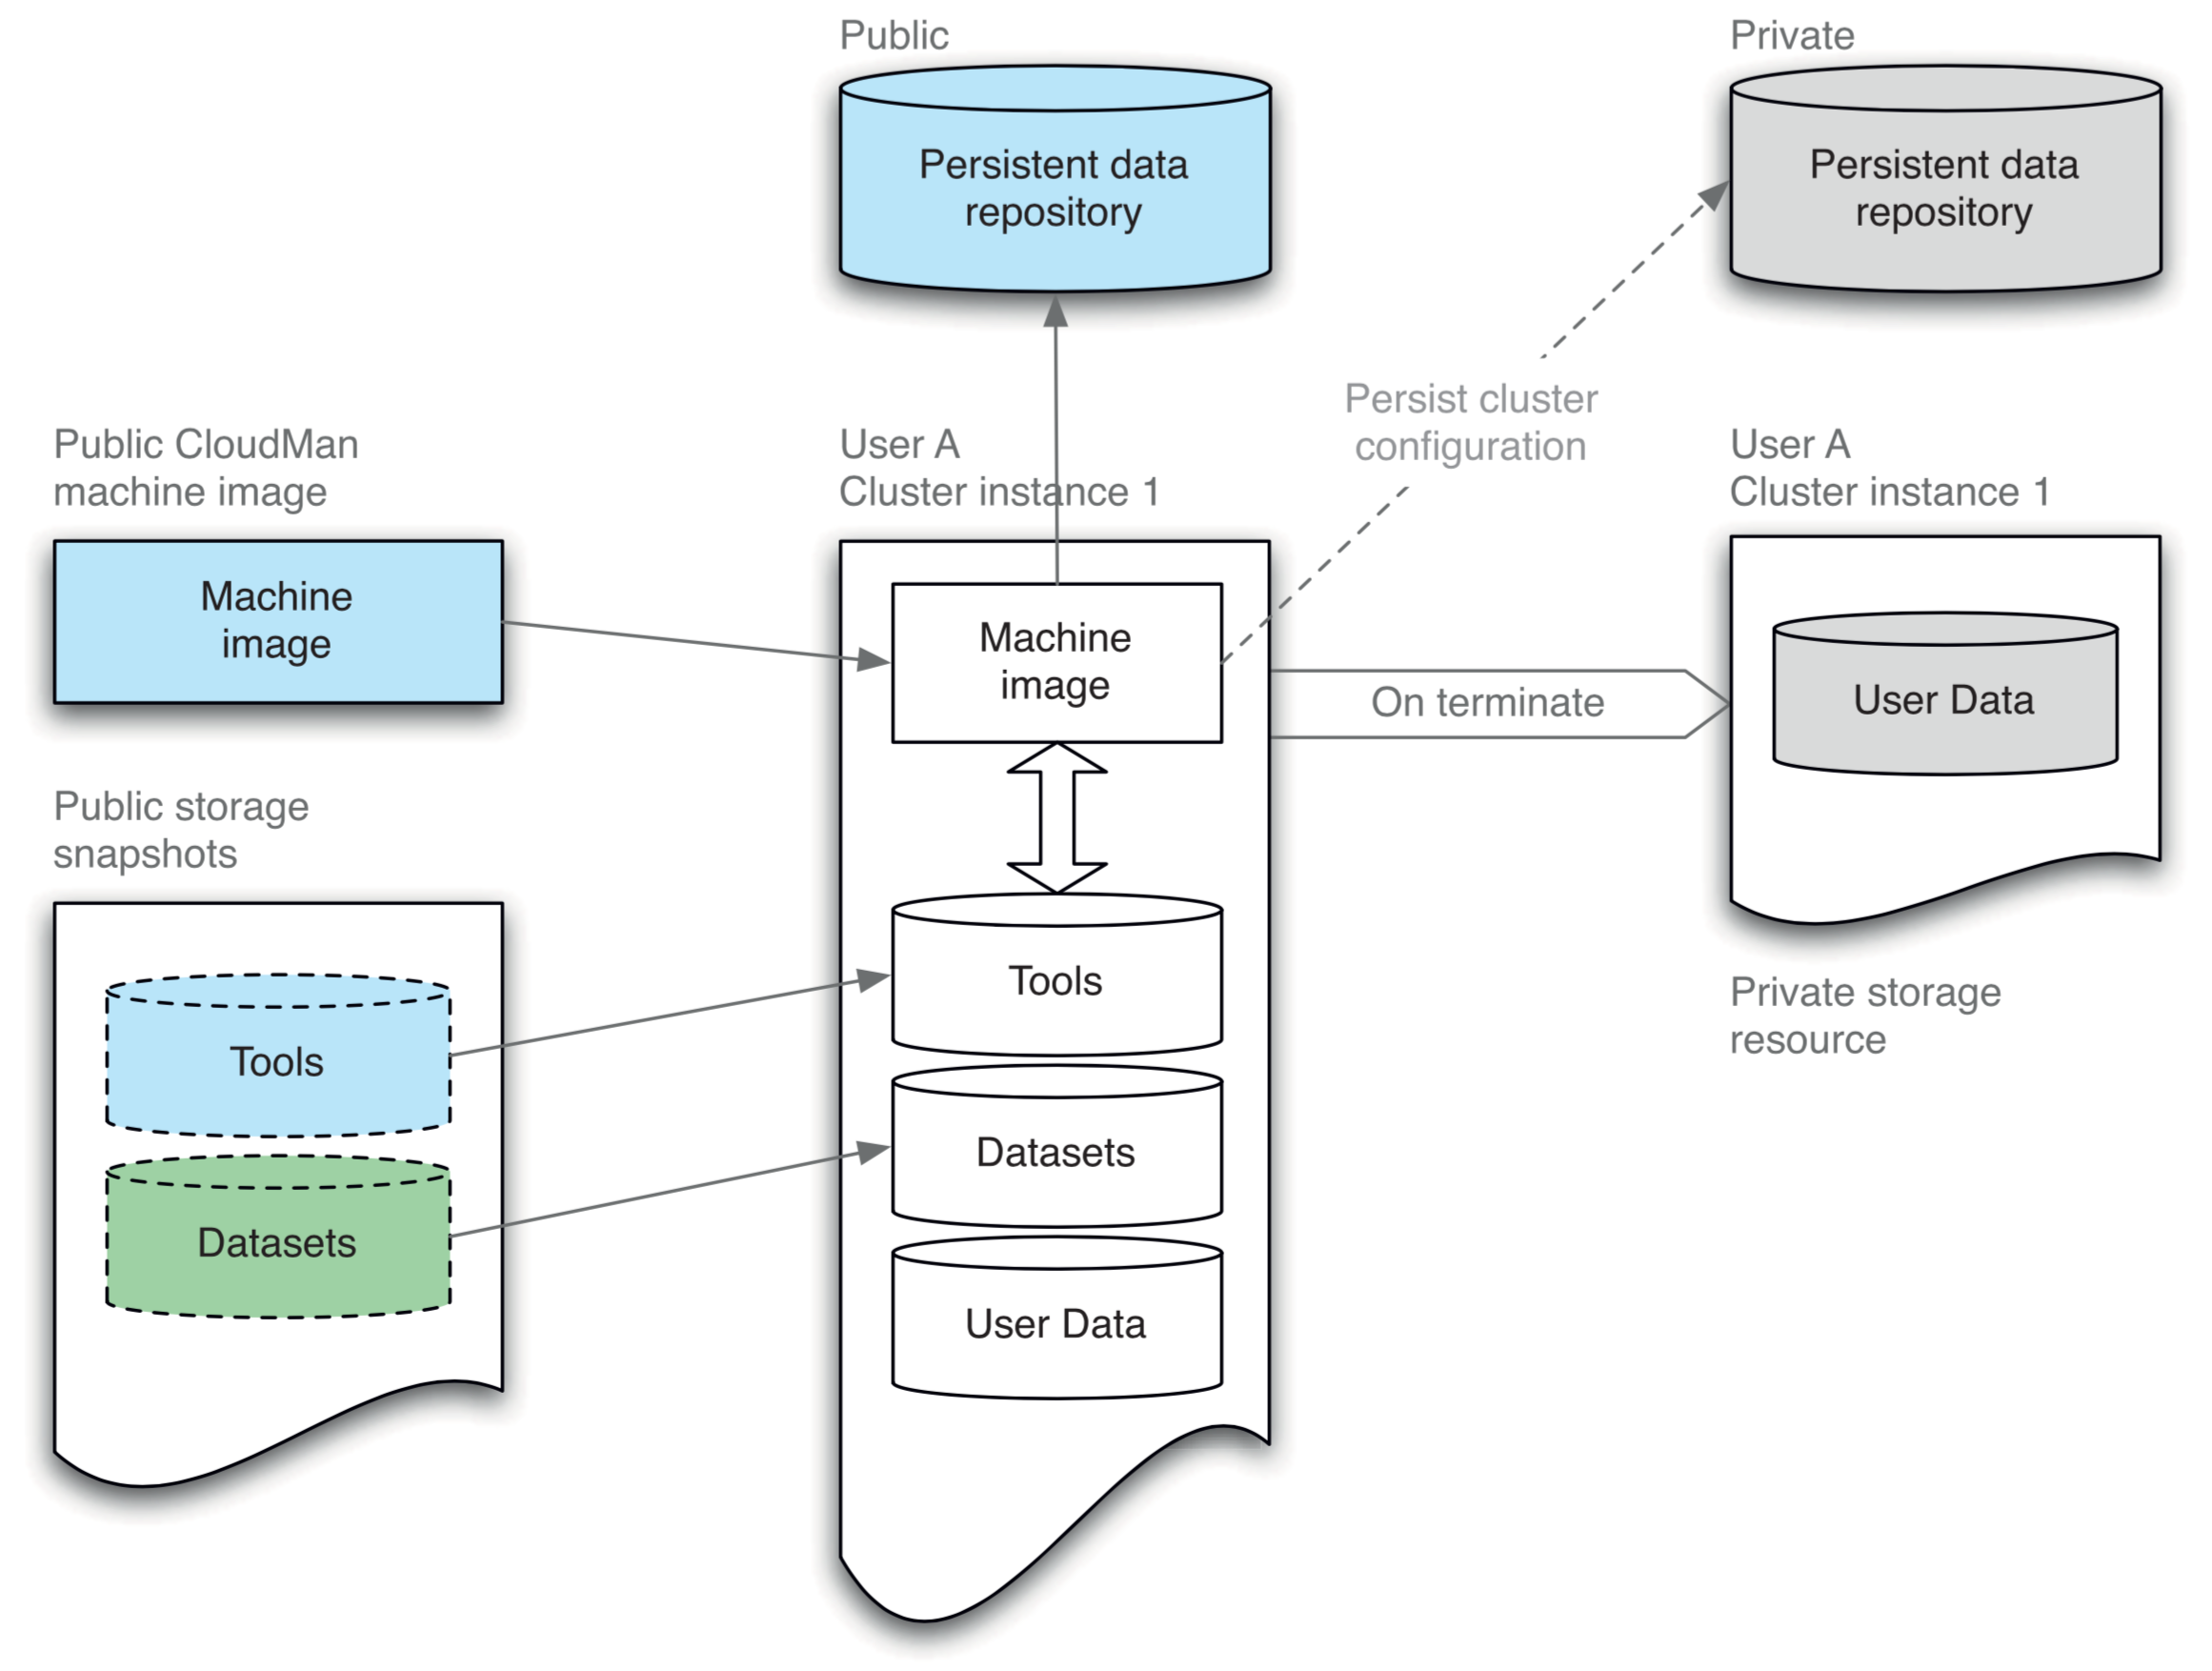
\includegraphics[scale=0.35]{figures/CloudManArch.png}
	\caption{CloudMan modular architecture \cite{Afgan2010}.}
	\label{CloudManArch}
\end{figure}

\subsection{Tavaxy}

Tavaxy \cite{Abouelhoda2012} was created from the desire to ease the sharing of scientific workflows between the increasingly large user bases of Taverna and Galaxy within the bioinformatics community. The limited interoperability between the two systems was caused by differences in workflow description languages, as well as execution engines and overall design. Tavaxy consolidates Taverna and Galaxy workflows to run and be edited in a single environment, encouraging the community to create composite routines with building blocks from both worlds.

Tavaxy focuses on efficiently and transparently delegating workload to grid and cloud platforms. It can run a cluster when it is provided with a distributed file system similar to NFS and a standard job scheduler like SGE. The preferred cloud platform is Amazon EC2 and provisioning extra resources is done via a simple web interface, operated similarly as for Taverna and Galaxy.

Three different modes are available for delegating computation to EC2:

\begin{itemize}
	\item \textit{Whole system instantiation}, where the user has no local version of Tavaxy installed and can bootstrap a new instance from a provided AMI. This will automatically create and configure a cluster that the user can control through a web console. Amazon S3 \cite{S3} is used for persistent storage of shared data in the cluster.
	\item \textit{Sub-workflow execution}, which presumes a local installation and Tavaxy used for workflow design and allows the user to create a cluster in the cloud from a more lightweight AMI wrapping the runtime environment. The local machine sends the workflows remotely for execution and waits for results of the run. The user has two options for transmitting the input data and persisting the results. The first option is to send Inputs along with the workflow definition to master node machine and save outputs manually to local storage. The alternative is to upload input data to S3 and configure the cluster to direct reads and writes to S3 directly. The general architecture for this mode of operation can be observed in Figure \ref{TavaxyArch}.
	\item \textit{Single task instantiation}, which is similar to sub-workflow execution, except that only a task in the workflow is delegated to the cloud.
\end{itemize}

\vspace{5mm}
\begin{figure}[h]
	\centering
		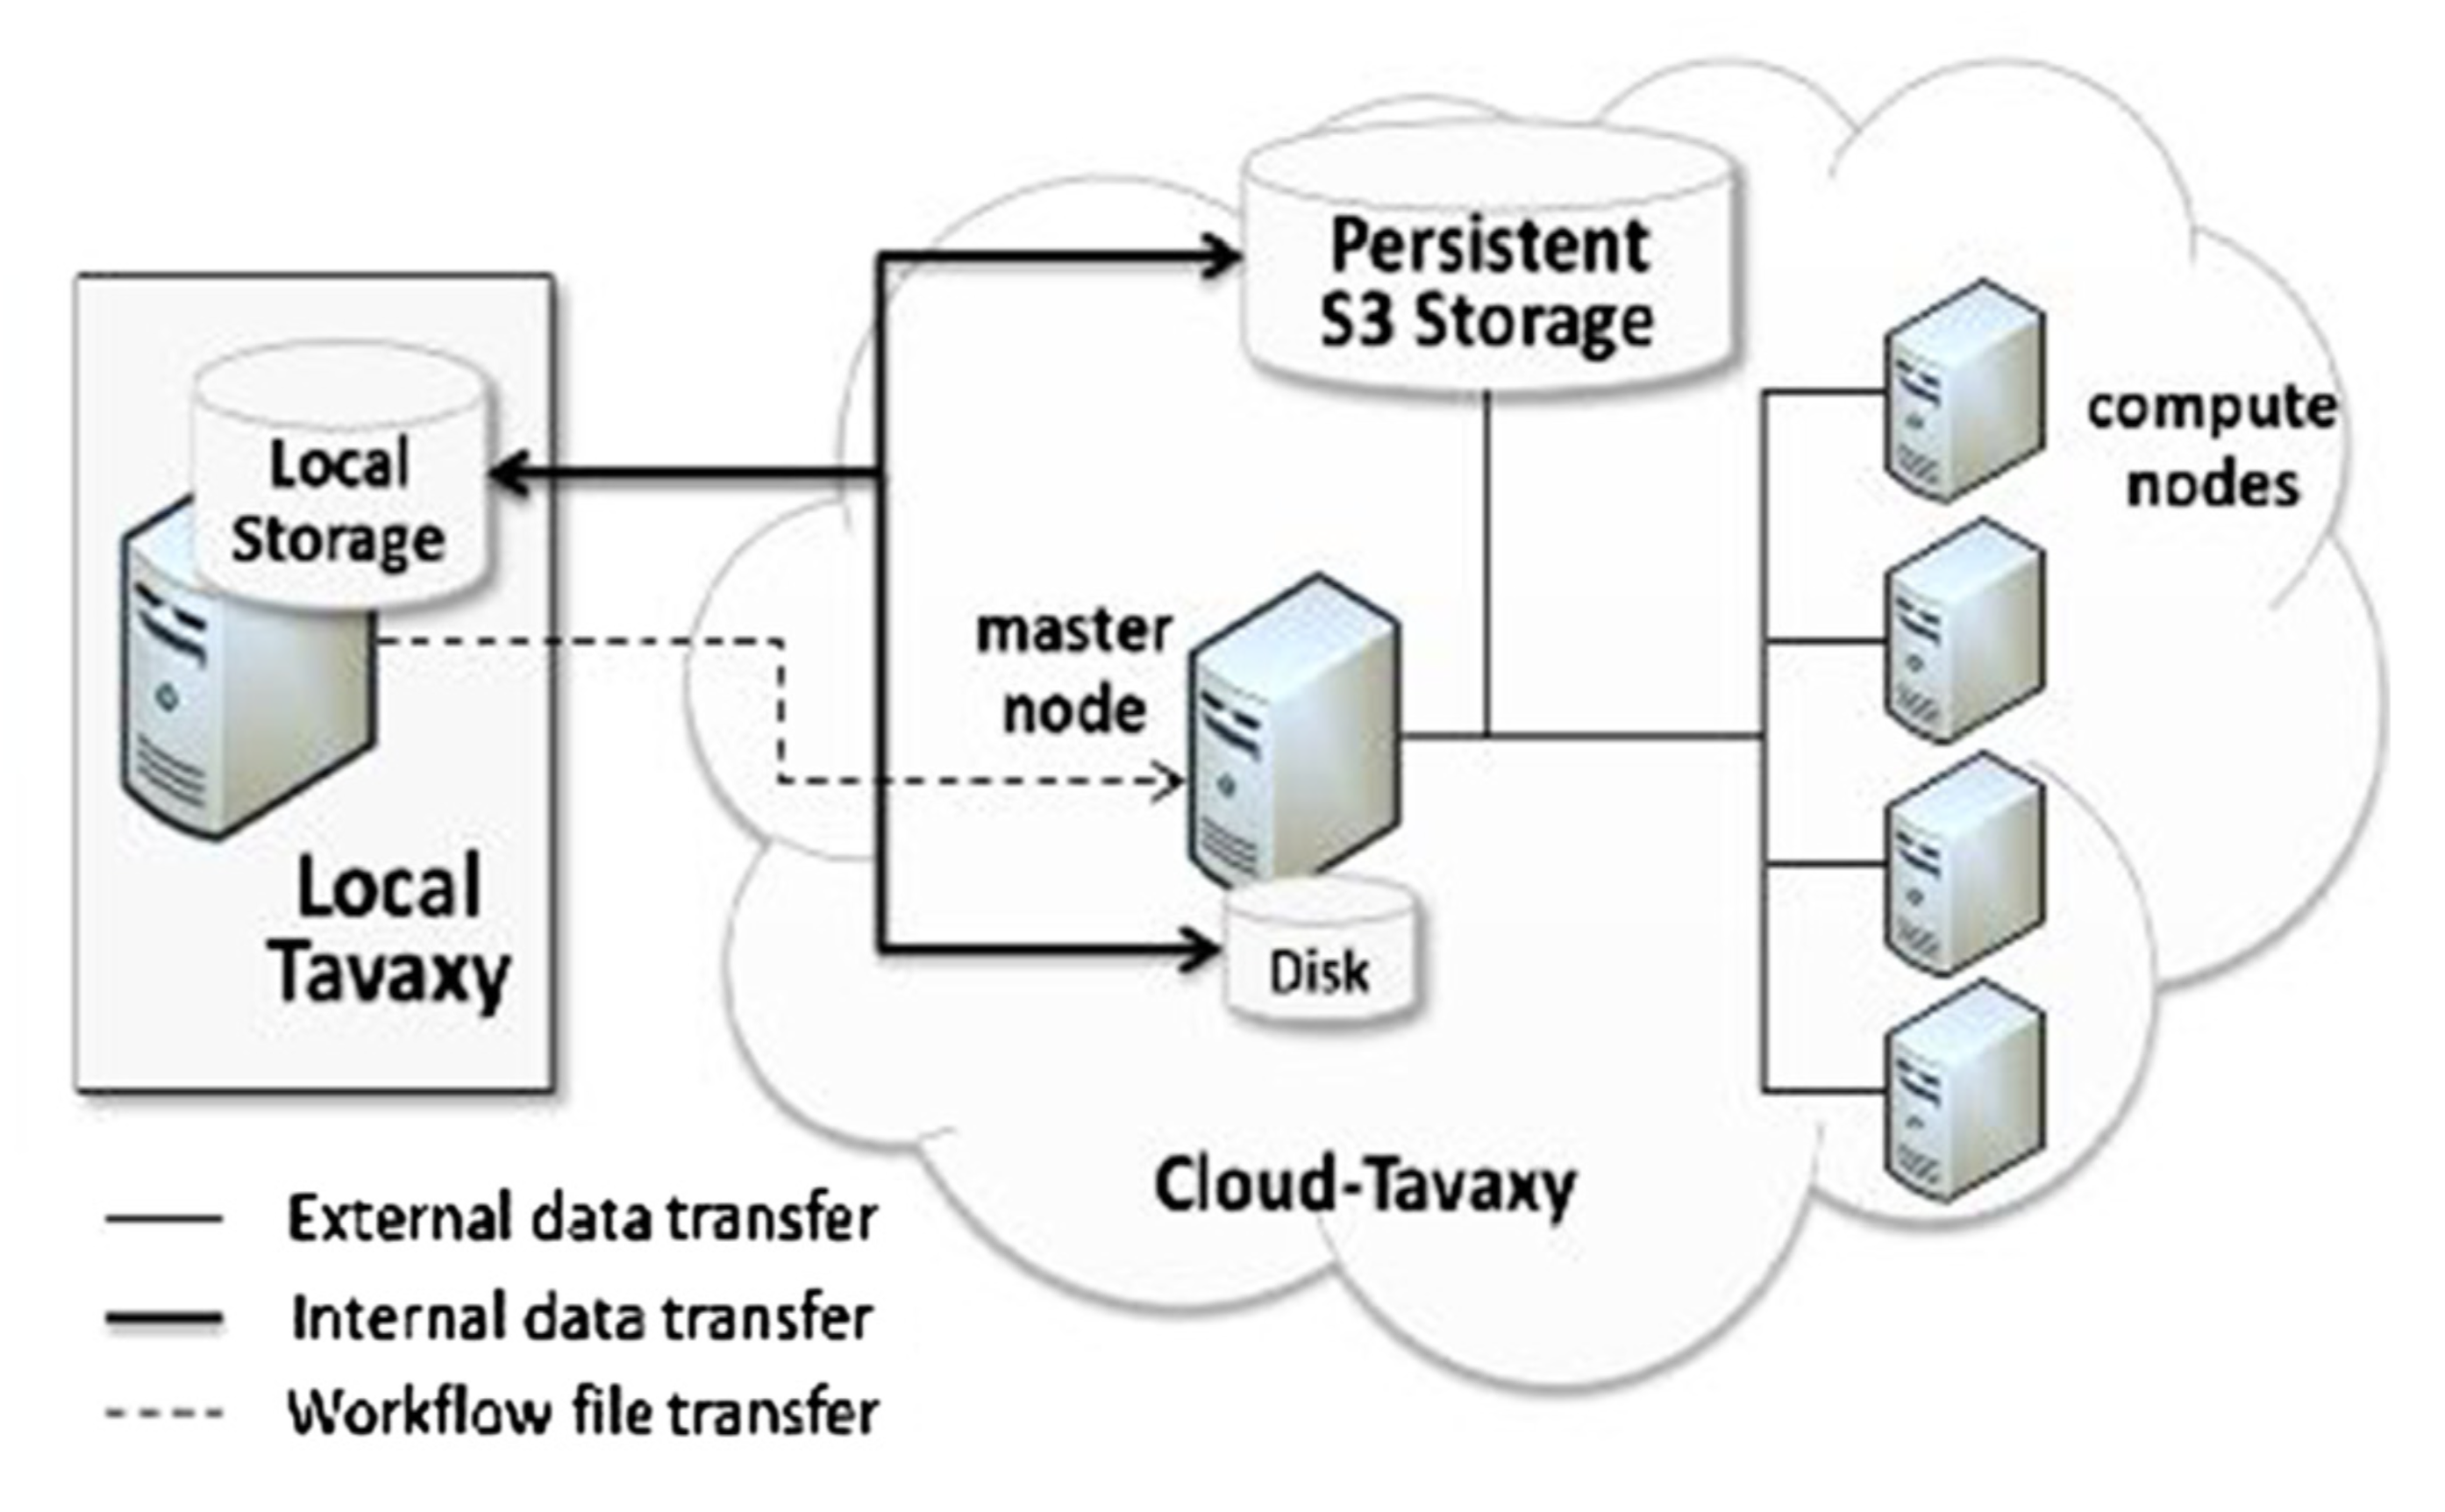
\includegraphics[scale=0.25]{figures/TavaxyArch.png}
	\caption{Tavaxy interaction between a local machine and Amazon EC2 \cite{Abouelhoda2012}.}
	\label{TavaxyArch}
\end{figure}

\subsection{Kepler}

Kepler \cite{Kepler} is one of the first general-purpose scientific workflow systems, recognising the need for transparent and simplified access to high performance computing platforms more than a decade ago. It also underlined concepts such as reusable and reproducible workflow runs, scalability of models, as well as fault tolerance and reliability in the context of remote execution \cite{Ludascher2006}.

The novelty of Kepler's design resides in the actor-oriented model. Actors are basic independent components representing either data sources or operations in the workflow. They are interconnected via channels and own receivers that handle their external communication, as well as input and output ports.

However, the execution model differs from standard systems in that its flow is not directed by the topology of the network. Instead, a special component named \textit{director} establishes the order of execution for actors, selects the operations they perform and orchestrates their communication by controlling their respective receivers \cite{Curcin2008}. This means that actors are not necessarily executed sequentially but are triggered by data received on incoming ports. Such as design reveals possibilities for concurrency semantics and renders the model fit for embedded systems simulations.

Although Kepler does not support execution on clusters in cloud environments out of the box, research groups using it have developed custom solutions to partially support this functionality. Wang and Altintas \cite{Wang2012} propose EC2 actors capable of managing Amazon virtual machines and suggest using StarCluster \cite{StarCluster} to build virtual clusters from the Kepler AMI they provide. This approach is sensible and can be used in conjunction with any other workflow systems, but is not readily available for Kepler at the moment.

\subsection{Pegasus}

Pegasus \cite{Pegasus} is a system that initially gained popularity for mapping complex workflows to resources resources in distributed environments without requiring input from the user \cite{Deelman2004}. Since its inception, many other similar applications have incorporated this feature, but Pegasus employs several optimisations that improve runtime performance and resource allocation.

Pegasus makes a clear distinction between high-level workflows defined by users from their actual executed form. Abstract workflows allow portability to many runtime platforms and free the user from explicitly indicating specific resources that should perform the work, while concrete workflows precisely bind execution stages to specific storage, computation, and network resources. This setup allows for multiple optimisations that would otherwise be impossible, particularly considering the fast dynamics of cloud and grid platforms. The latest release of Pegasus relies on four essential components \cite{Deelman2013, Deelman2016}:

\begin{itemize}
	\item The \textit{mapper} receives an abstract workflow as an input and produces a concrete workflow, defining the software and hardware requirements of the computation. Additionally, it performs metadata processing to enable data provenance tracking and modifies the structure of the workflow by grouping suitable tasks.
	\item The \textit{workflow engine} ensures the execution in topological order. This responsibility is delegated to DAGMan \cite{DAGMan}, a meta-scheduler that runs on top of HTCondor \cite{HTCondor} and allows ready jobs to be run.
	\item The HTCondor \textit{job scheduler} manages the queue of individual jobs. It supervises the execution and restarts task runs in the case of failures.
	\item The \textit{workflow monitor} is a daemon that parses output logs and notifies the end-user on the status of the submission.
\end{itemize}

Pegasus performs most of its important optimisations at the mapping stage, since this is the point where the workflow is broken down into single tasks. The improvements with significant impact on performance concern the following aspects \cite{Deelman2016}

\begin{itemize}
	\item \textit{Data movement}. This refers to ensuring that data required by a job is collocated with resources where it is executed. For example, copying input data from a user's local server to EBS is highly preferred when running jobs on EC2 because Amazon guarantees low latency when accessing its own storage systems.
	\item \textit{Data reuse}. Pegasus is able to reuse intermediate results of the workflow that have already been computed during previous runs of the workflow if the definitions of the tasks and input data have not changed. The process requires careful coordination with the \textit{data cleanup} phase in order to simultaneously leverage already known results and avoid wasting storage capacity.
	\item \textit{Job clustering}. For many short-lived jobs, orchestrating the transfer of task results across machines in a cluster and long queueing times can incur high latency costs. Grouping related tasks into larger entities helps alleviate this problem by reducing the load on the machine that hosts the job submission system. This strategy also improves the overall performance of workflows with a large number of tasks by over 90\%, as previous studies have shown \cite{Deelman2010, Singh2008}. \textit{Level-based horizontal clustering} (Figure \ref{HorizontalClustering}) and \textit{label-based clustering} (Figure \ref{LabelClustering}) are some of the most effective strategies, although the latter requires users to explicitly label tasks when defining the workflow \cite{Deelman2013}.
\end{itemize}
	
\vspace{5mm}
\begin{figure}[h]
	\centering
		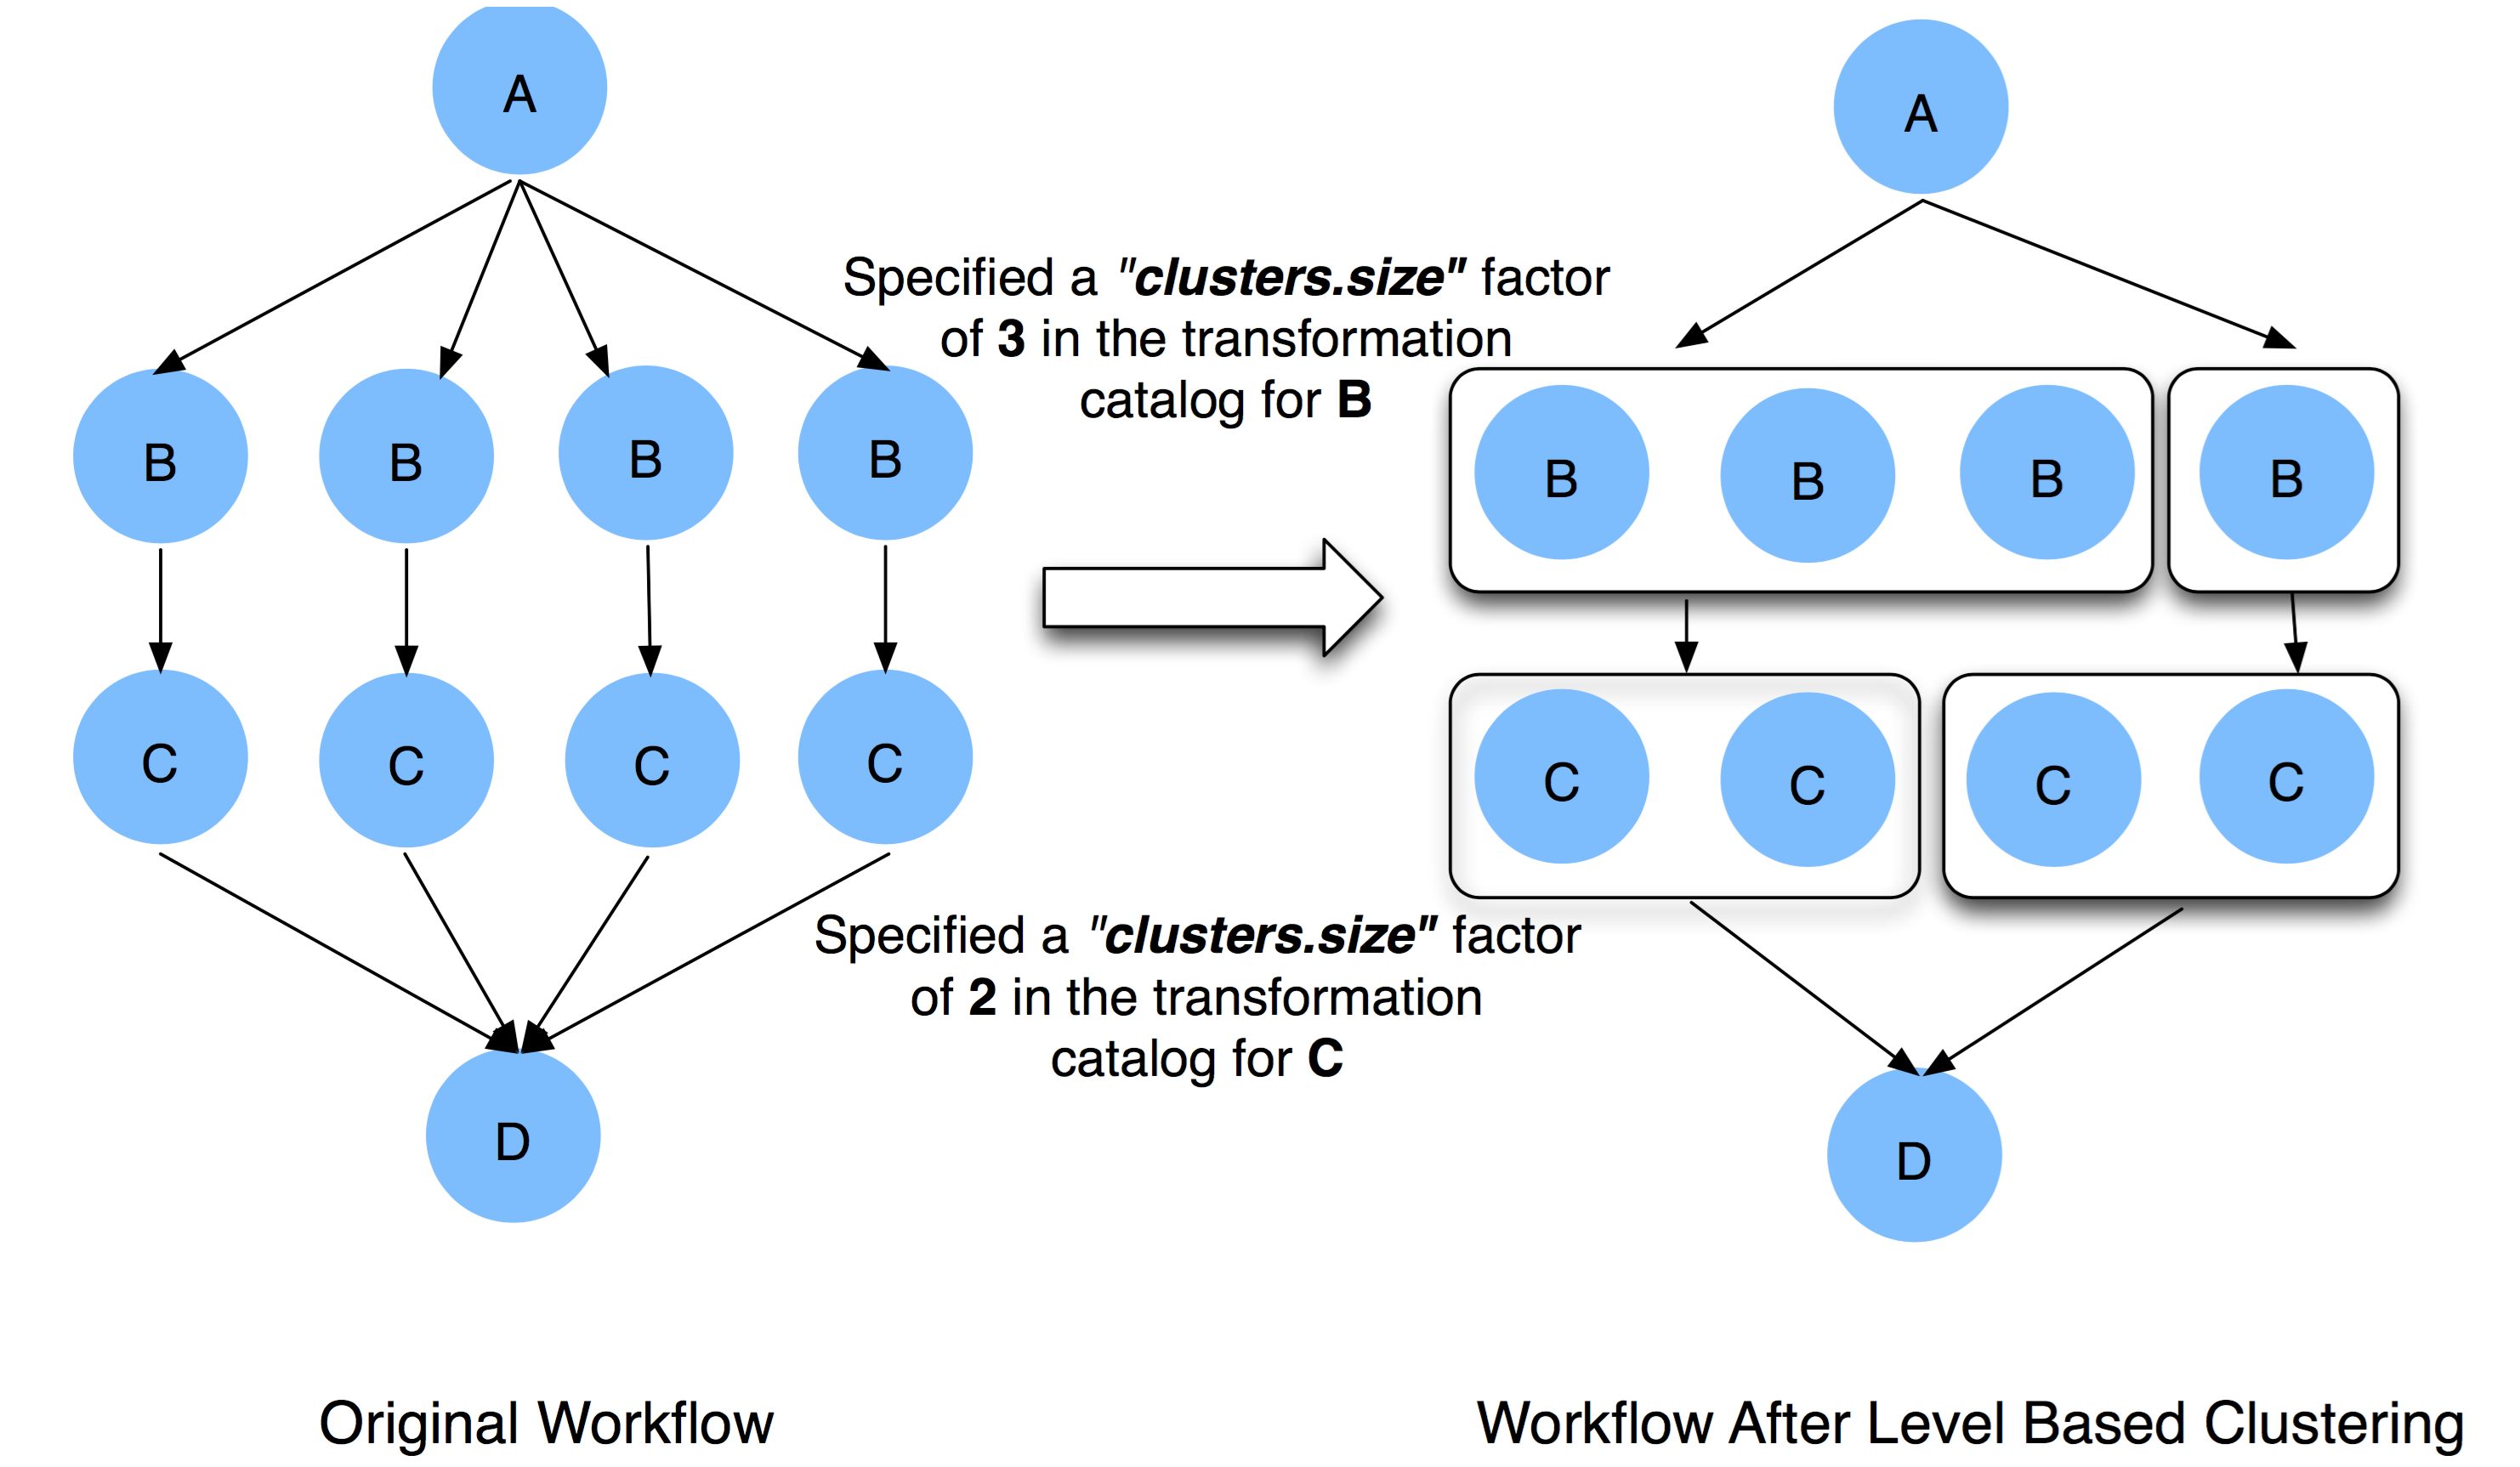
\includegraphics[scale=0.23]{figures/HorizontalClustering.png}
	\caption{Level-based horizontal clustering targeting parallelisable tasks \cite{Deelman2013}.}
	\label{HorizontalClustering}
\end{figure}

\vspace{6mm}
\begin{figure}[h]
	\centering
		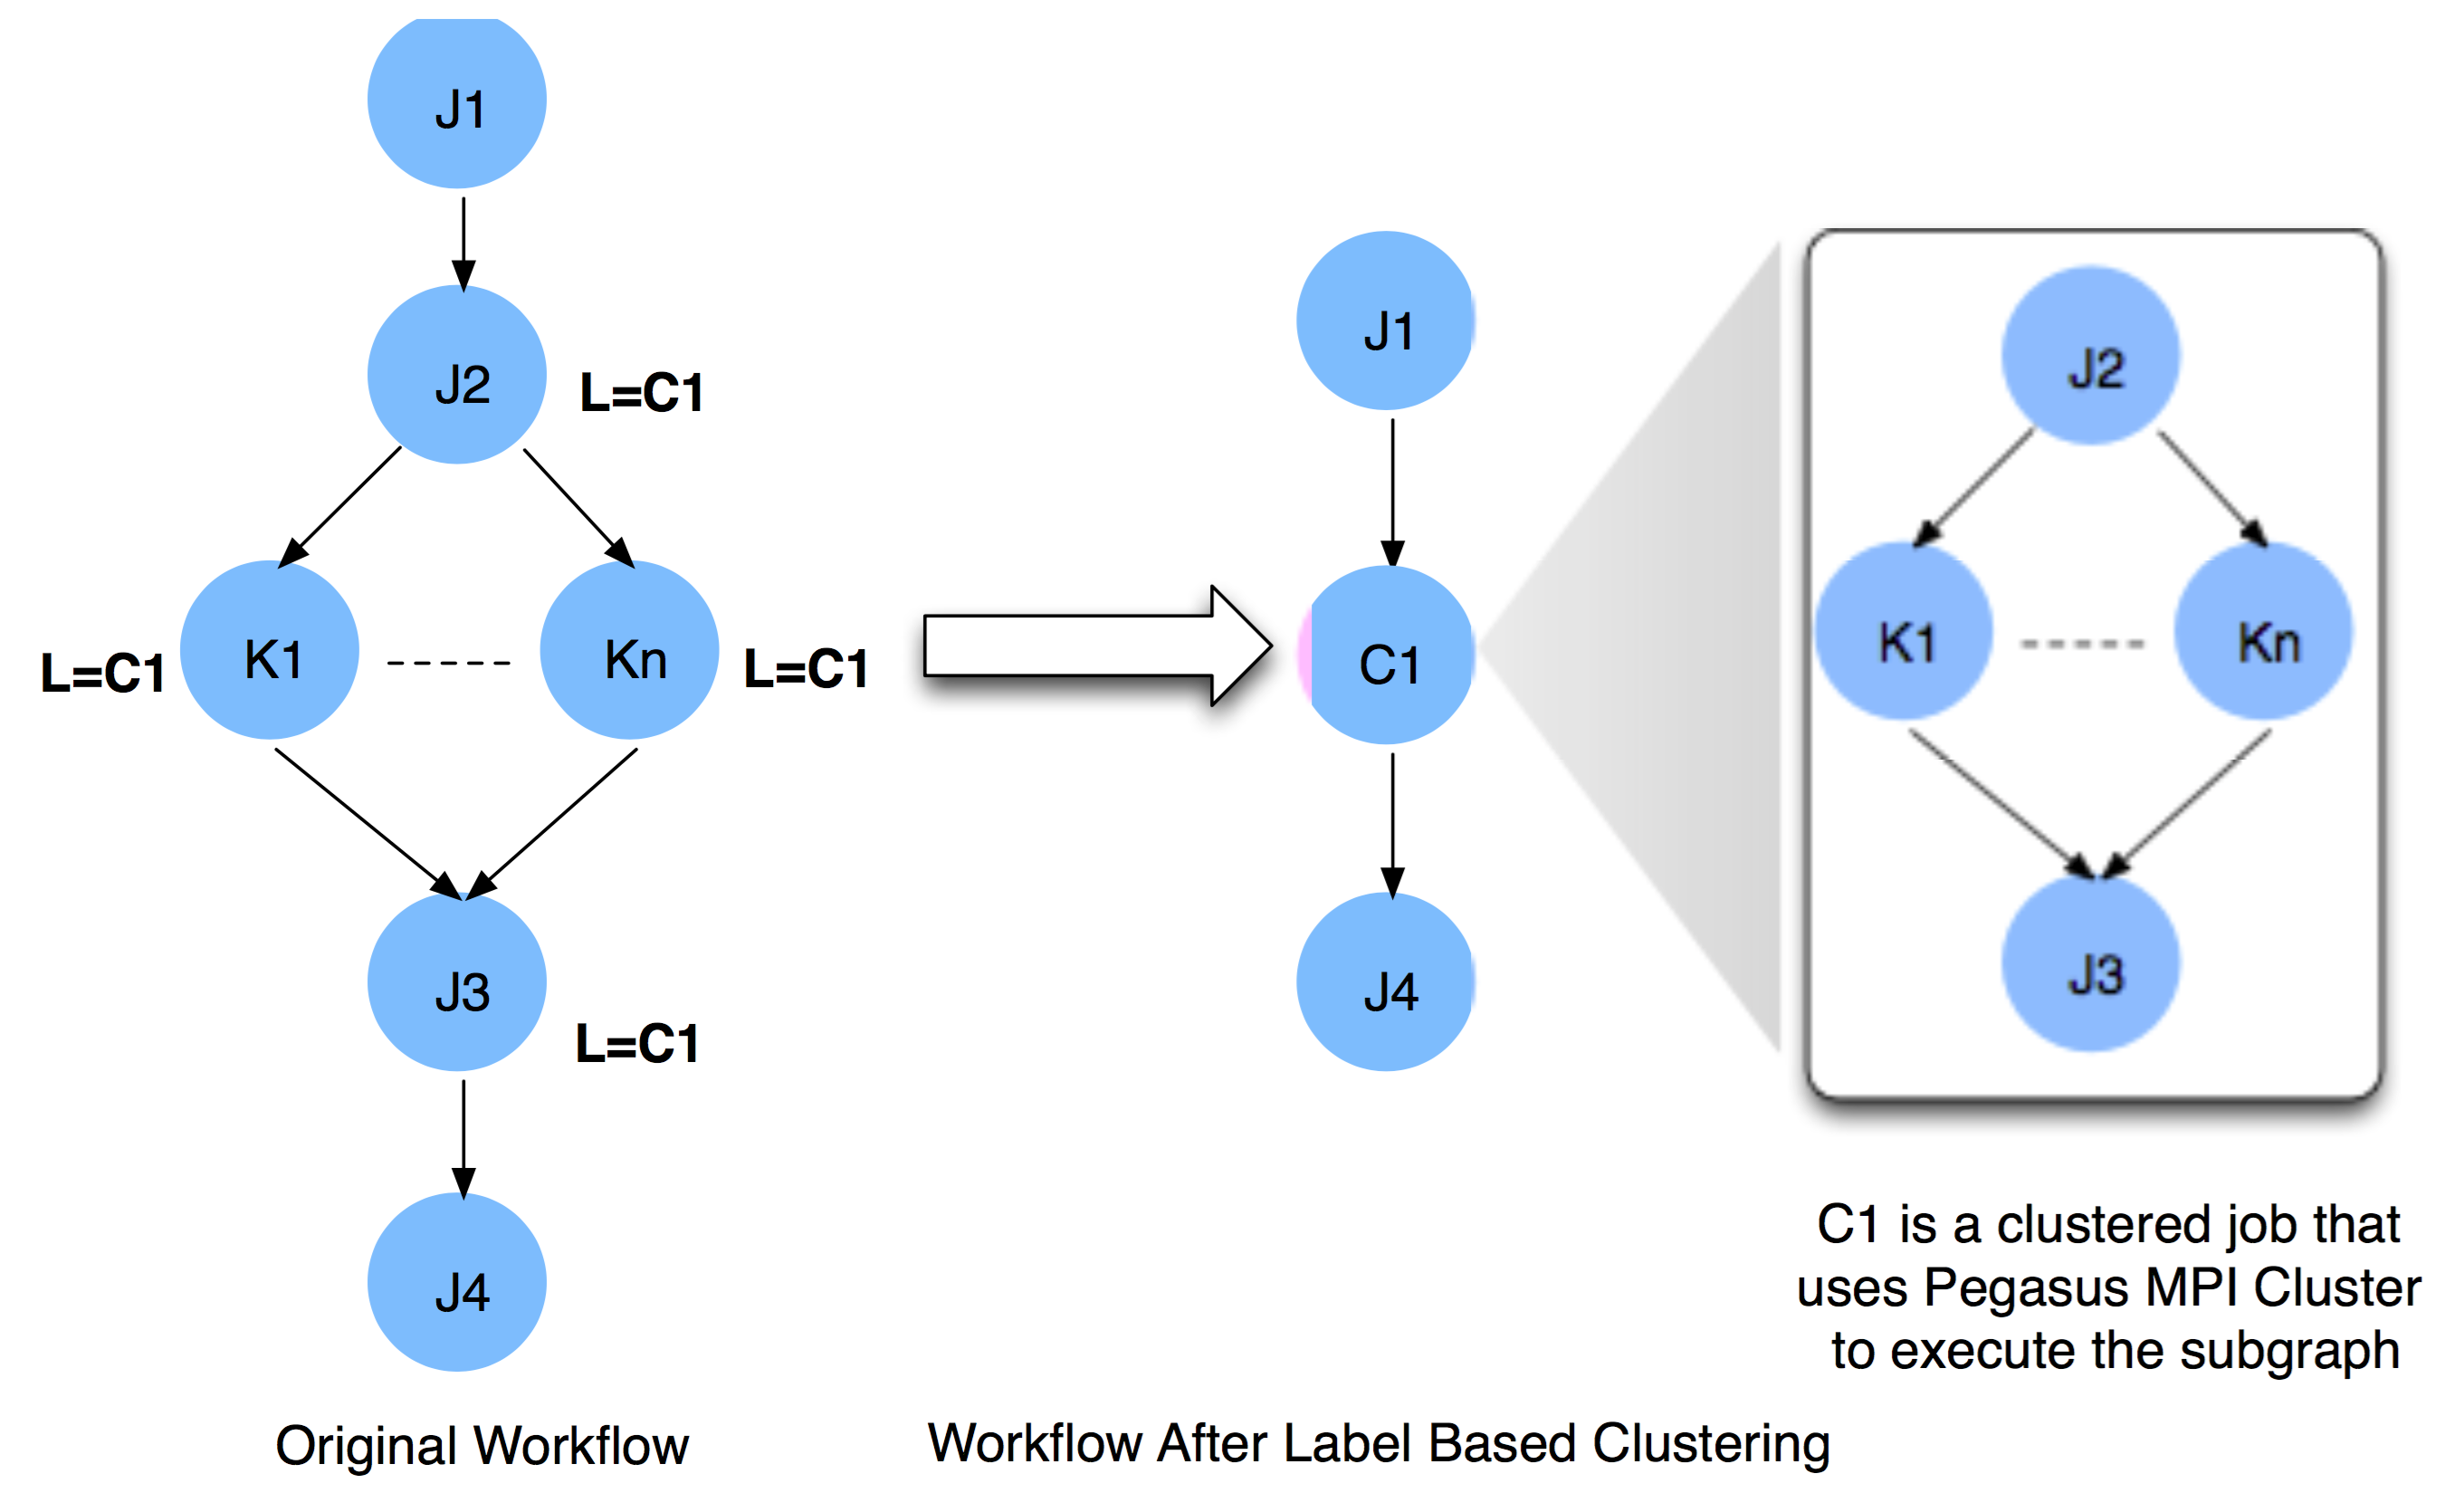
\includegraphics[scale=0.23]{figures/LabelClustering.png}
	\caption{Label-based clustering \cite{Deelman2013}.}
	\label{LabelClustering}
\end{figure}

Although all the optimisations and design ideas discussed above apply to all distributed execution platforms, earlier deployments of Pegasus have confirmed several advantages of cloud environments. These include on-demand provisioning of resources and ability to easily ensure consistency of software installed on all the machines in a fleet \cite{Deelman2016}. 

However, further development of workflow management systems is needed in order to fully exploit cloud features such as automatic scaling of available resources. The main problem is that the load of instances occurs in the case of long-running jobs. Indeed, upscaling usually leaves unused extra resources, while downscaling is even more challenging because long individual tasks cannot be split up any further. Basic solutions involve only allowing automatic scaling on idle instances or when having many short-lived jobs, but this is definitely an area open to future work.

Despite the trend towards cloud-based systems, the process of running Pegasus workflows in the cloud has still not been fully automated. Users are required to manually configure the job submission host and worker nodes to run the required software. The technical barrier for harnessing the cloud from Pegasus is higher than grid-based options, that are usually professionally managed.

\todo[inline]{@Adrian: not sure to understand this last sentence (even after my change). Do you mean that it's easier to use Pegasus with grids than clouds?}

\section{Cluster Deployment on Clouds}

\subsection{Chronos}

\subsection{Mesosphere}

\subsection{CometCloud}

\subsection{elasticluster}

\subsection{SWF}

\subsection{CfnCluster}

\subsection{Starcluster}

\chapter{Project Plan}



\begin{itemize}
	\item Minimum viable product
	\item Exact implementation goals
	\item Timeline
\end{itemize}

\chapter{Evaluation Plan}

\begin{itemize}
	\item Evaluation at each milestone
	\item Benchmarks (against known workflow engines from bioinformatics / biomedical imaging world)
	\item Comparisons with performance at start of project
	\item Show ease of running on different environments
	\item Evaluate
\end{itemize}

\listoftodos

\bibliography{MEngProject}

\end{document}